\documentclass{article}
\usepackage[paperletter]{geometry}
\geometry{top=1.0in, bottom=1.0in, left=1.0in, right=1.0in}
\usepackage[utf8]{inputenc}
\usepackage{cancel}
\usepackage{tikz}
\usepackage{siunitx}
\usepackage{amsmath}
\usepackage{mathdots}
\usepackage{yhmath}
\usepackage{color}
\usepackage{array}
\usepackage{multirow}
\usepackage{amssymb}
\usepackage{gensymb}
\usepackage{tabularx}
\usepackage{booktabs}
\usepackage{booktabs}
\usepackage{float}
\usepackage{multicol}
\usetikzlibrary{fadings}
\usetikzlibrary{patterns}
\usetikzlibrary{shadows.blur}
\usepackage[symbol]{footmisc}
\renewcommand*{\thefootnote}{\fnsymbol{footnote}}
\usepackage{everysel}
\usepackage{ragged2e}
\renewcommand*\familydefault{\ttdefault}
\EverySelectfont{%
\fontdimen2\font=0.4em% interword space
\fontdimen3\font=0.2em% interword stretch
\fontdimen4\font=0.1em% interword shrink
\fontdimen7\font=0.1em% extra space
\hyphenchar\font=`\-% to allow hyphenation
}
\pagenumbering{gobble}
\title{Ice Puck Sliding Lab \\ AP \textsc{Physics} $-$ C}
\author{Michael \textsc{Brodskiy}}
\date{September 21, 2020}

\begin{document}

\maketitle
\begin{center}
\begin{tabular}{l r}
\underline{Date Performed}: & September 2020 \\\\ % Date the experiment was performed
\underline{Partners}: & Andrew Wang \\ & Yiying Zhang \\ & Salih Saygi \\\\
\underline{Instructor}: & Mrs. Morse \\\\\\\\\\ % Instructor/supervisor
\end{tabular}
\end{center}
\newpage
    
\section{Gathered Data}

\begin{enumerate}

  \item \begin{tabular}{|l|l|}

  \hline
  Time $[\si{\second}]$ & Distance $[\si{\centi\meter}]$ \\
  \hline
   0 & 0  \\
  \hline
  .1 & 5  \\
  \hline
  .2 & 13 \\
  \hline
  .3 & 26 \\
  \hline
  .4 & 44 \\
  \hline
  .5 & 66 \\
  \hline
  .6 & 93 \\
  \hline
  .7 & 124\\
  \hline
  .8 & 159\\
  \hline

\end{tabular}

\item Mass = $420[\si{\gram}]$

\item Angle = $28\degree$

\end{enumerate}

\section{Graphs}

\begin{figure}[htpb]
  \centering
  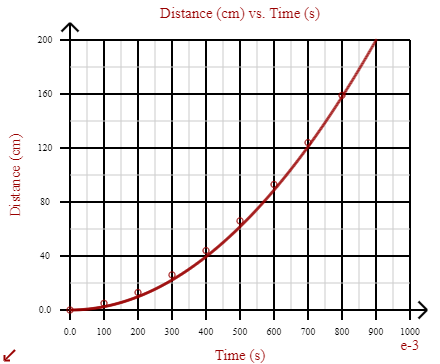
\includegraphics[width=.7\textwidth]{Figures/Curved.png}
  \caption{Non-linearized Data}
\end{figure}

\begin{figure}[htpb]
  \centering
  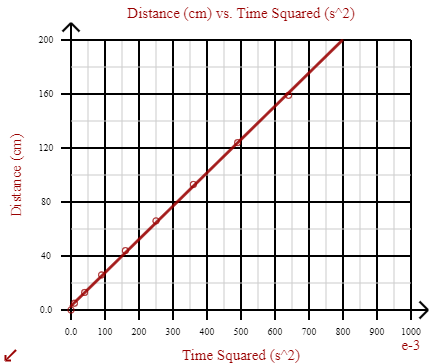
\includegraphics[width=.7\textwidth]{Figures/Linear.png}
  \caption{Linearized Data, $d=246.7t^2+2.978$}
\end{figure}

\newpage

\section{Mathematical Analysis}

$$\text{The equation yielded by the linearized graph is: } d=246.7t^2+2.978 \text{ or } d=246.7s+2.978, $$
$$\text{where variables substitution } (s = t^2) \text{ is used to keep the function linear.}$$
$$\text{Thus, the slope is } 246.7\left[\frac{\si{\centi\meter}}{\si{\second\squared}}\right], \text{ as this value represents the acceleration of the ice puck.}$$

\end{document}
